\documentclass[11pt]{article}
\usepackage[toc,page]{appendix}
\usepackage{amsmath, amssymb}
\usepackage[style=apa,backend=biber]{biblatex}
\addbibresource{references.bib}
\usepackage{graphicx}
\usepackage{tikz}
\usetikzlibrary{automata,positioning,shapes.geometric, arrows.meta, fit, backgrounds, calc, chains}
%\usepackage{kpfonts}
\usepackage{float}
\usepackage[margin=1in]{geometry}
\usepackage{cancel}
\usepackage{epsfig}
\usepackage{tikz-3dplot}
\usepackage{darkmode}
\usepackage{dirtytalk}
\usepackage{longtable,booktabs,array}
\usepackage{calc} % for calculating minipage widths
\usepackage{etoolbox}
\usepackage{hyperref}
\hypersetup{
    colorlinks=true,
    linkcolor=blue,
    filecolor=magenta,
    urlcolor=cyan,
    pdftitle={Hermeneutic Calculator},
    citecolor=blue,
}

\urlstyle{same}

% Optional: define some custom colors
\definecolor{sliceRed}{RGB}{225,224,91}
\definecolor{linkYellow}{RGB}{255,215,0}
\tdplotsetmaincoords{70}{110}

\title{Multiplication Strategies: Strategic Counting}
\author{Theodore M. Savich}
\date{}

\begin{document}
\maketitle

Strategy descriptions and examples adapted from \textcite{HackenbergCourseNotes}. 

This method uses additive techniques—like Rearranging Ones to Make Bases (RMB), Chunking, or Rounding—to manage two distinct types of units while calculating the total number of items. The goal isn’t to count one by one but to employ a more efficient grouping strategy. Nonetheless, each group is still added sequentially, one at a time.


For example, if you have six groups of 7, you could use rearranging to make bases several times -- keeping track of the number of groups and the total number of items in each group -- to obtain 42. 

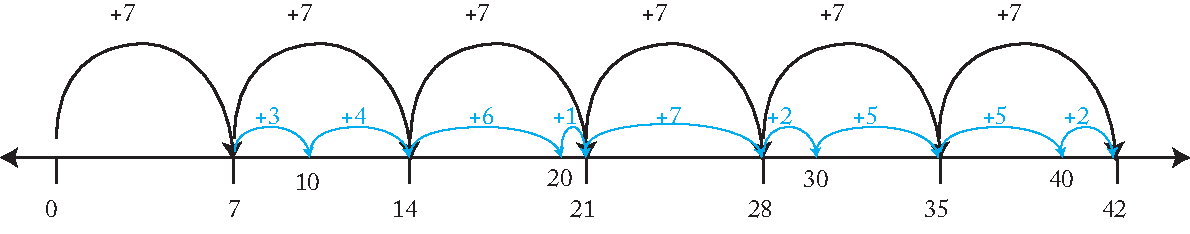
\includegraphics[width=.8\textwidth]{images/Easy_Pictures/SMR_Multiplication_Strategic_Counting_RMB/PDF/SMR_MULTIPLICATION_Strategic_Counting.pdf}

Or, for the same problem, you could pretend to add 10, then adjust back by three, over and over again until you reach the total.

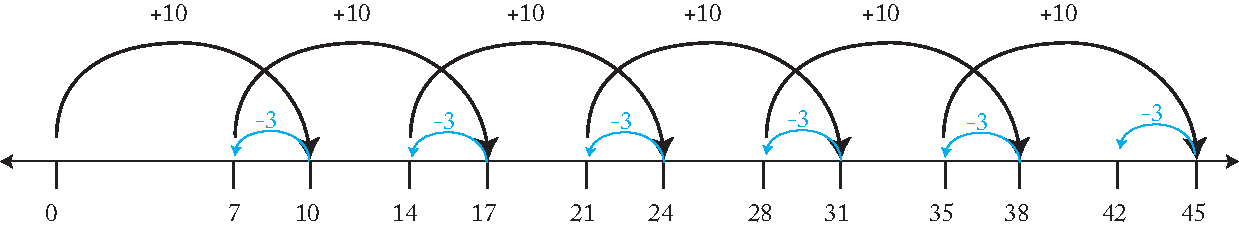
\includegraphics[width=.8\textwidth]{images/Easy_Pictures/SMR_Multiplication_Strategic_Counting_Rounding/PDF/SMR_Multiplication_Strategic_Counting_Rounding.pdf}






\subsubsection*{Description of Strategy}
\begin{itemize}
    \item \textbf{Objective:} Use any of several \textbf{additive} strategies (for example, rearranging ones to make bases, chunking, rounding, etc.) to add the group size without counting each item by ones.
    \item \textbf{Method:} Instead of incrementing one by one, interpret the multiplication problem as repeated addition of the group size, then apply one of the \textbf{efficient} addition strategies for each step.
\end{itemize}

\subsubsection*{Automaton Type}
\textbf{Finite State Automaton with Registers (Counters)}. Below is a high-level representation. A two-stack automaton approach is described later.

\subsubsection*{Formal Description of a High-Level FSA}

We define the automaton as:
\[
M = (Q,\, \Sigma,\, \delta,\, q_{0/accept},\, F,\, V)
\]
where:
\begin{itemize}
    \item \(Q = \{q_{0/accept},\, q_{\text{add\_group}},\, q_{\text{next\_group}}\}\).
    \item \(q_{0/accept}\) is both the start and accept state.
    \item \(F = \{q_{0/accept}\}\).
    \item \(V = \{\text{GroupCounter}(G),\ \text{Total}(T),\ \text{GroupSize}(S),\ \text{TotalGroups}(N)\}\).
\end{itemize}

\begin{enumerate}
    \item \textbf{Initialization:} From \(q_{0/accept}\), read \(S\) and \(N\). Set \(G=0\) and \(T=0\), then transition to \(q_{\text{add\_group}}\).
    \item \textbf{Add the Group Size:} In \(q_{\text{add\_group}}\), add \(S\) to \(T\). (This step uses a chosen addition strategy like chunking or rearranging.)
    \item \textbf{Next Group:} If \(G < N\), transition to \(q_{\text{next\_group}}\), increment \(G\), and return to \(q_{\text{add\_group}}\). If \(G = N\), move back to \(q_{0/accept}\).
\end{enumerate}

\subsubsection*{Automaton Diagram for Strategic Counting (High-Level)}
\begin{figure}[H]
\centering
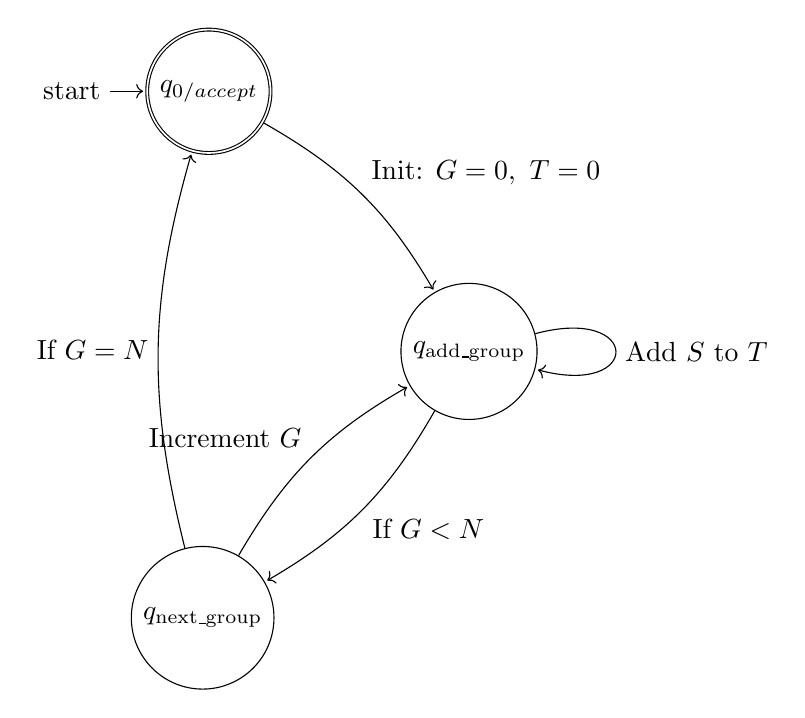
\begin{tikzpicture}[shorten >=1pt, auto, node distance=3cm, every state/.style={minimum size=1cm}]
    \node[state, initial, accepting] (q0) {${q_{0/accept}}$};
    \node[state] (q1) [below right=of q0] {${q_{\text{add\_group}}}$};
    \node[state] (q2) [below left=of q1] {${q_{\text{next\_group}}}$};

    \path[->]
        (q0) edge[bend left=15] 
            node[align=center]{Init: $G=0,\ T=0$} 
            (q1)
        (q1) edge[loop right] 
            node[align=center]{Add $S$ to $T$} 
            (q1)
        (q1) edge[bend left=15] 
            node[align=center]{If $G < N$} 
            (q2)
        (q2) edge[bend left=15] 
            node[align=center]{Increment $G$} 
            (q1)
        (q2) edge[bend left=15] 
            node[align=center]{If $G = N$} 
            (q0);
\end{tikzpicture}
\caption{High-level FSA for Multiplying via Strategic Counting}
\end{figure}

\subsection*{Two-Stack Automaton (2-PDA) for Strategic Counting}

Rather than a single FSA, we can compose two distinct Pushdown Automata:
\begin{itemize}
    \item \textbf{Sub-PDA\(_1\)}: Manages how many groups are left to process. 
    \item \textbf{Sub-PDA\(_2\)}: Implements one of the sophisticated addition strategies for adding the group size to the running total.
\end{itemize}

A single-stack PDA cannot hold both sub-automata memories separately. Therefore, we move to a \textbf{two-stack automaton} (2-PDA), which formally:
\[
P_{\times} = (Q_1 \times Q_2,\ \Sigma,\ \Gamma_1,\ \Gamma_2,\ \delta_{\times},\ (q_{1,0}, q_{2,0}),\ F_1 \times F_2).
\]
Here, \(\Gamma_1\) is the stack alphabet for the group-counting sub-PDA, and \(\Gamma_2\) is the alphabet for the addition-strategy sub-PDA.

\begin{figure}[H]
\centering
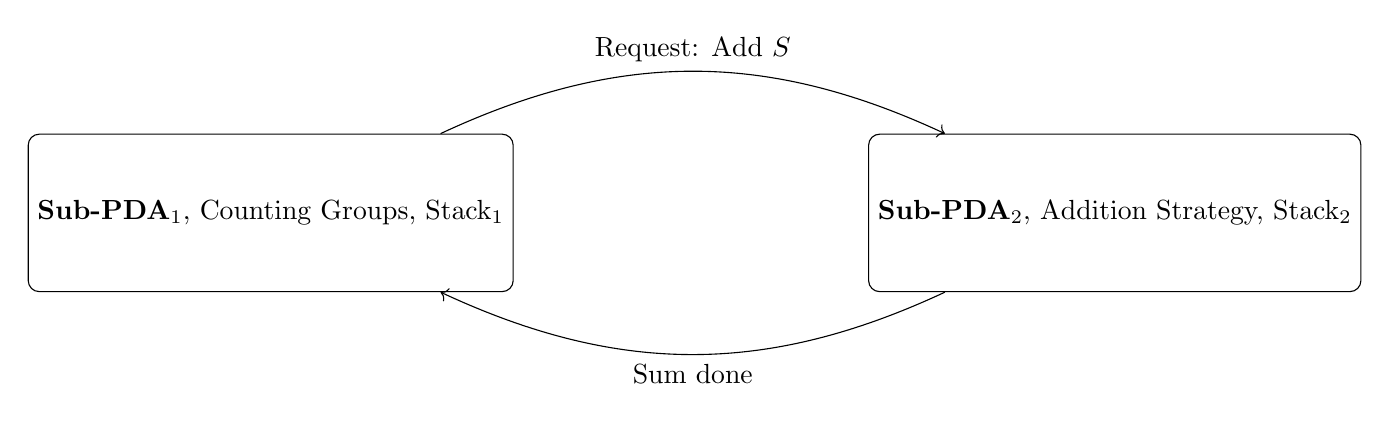
\begin{tikzpicture}[->, node distance=4.5cm, auto]
    \node[draw, rectangle, rounded corners, minimum width=3cm, minimum height=2cm] (gPDA) 
        {\textbf{Sub-PDA\(_1\)}, Counting Groups, Stack\(_1\)};
    \node[draw, rectangle, rounded corners, minimum width=3cm, minimum height=2cm, right=of gPDA] (iPDA)
        {\textbf{Sub-PDA\(_2\)}, Addition Strategy, Stack\(_2\)};

    \path (gPDA) edge[bend left=25] node[align=center]{Request: Add $S$} (iPDA)
          (iPDA) edge[bend left=25] node[align=center]{Sum done} (gPDA);
\end{tikzpicture}
\caption{Two-Stack Composition for Strategic Counting}
\end{figure}

\textbf{How it Works:}
\begin{enumerate}
    \item \textbf{Initialize}: Sub-PDA\(_1\) stores the total number of groups \(N\) in Stack\(_1\). Sub-PDA\(_2\) sets up partial sum \(T=0\) in Stack\(_2\).
    \item \textbf{Repeated Addition}: 
        \begin{itemize}
            \item Sub-PDA\(_1\) checks if there is another group left (e.g., by decrementing \(N\)). 
            \item If yes, it triggers Sub-PDA\(_2\) to add \(S\) to \(T\) using a more advanced approach (chunking, rearranging to make bases, etc.).
            \item Once Sub-PDA\(_2\) completes the addition, control goes back to Sub-PDA\(_1\).
        \end{itemize}
    \item \textbf{Accept}: When Sub-PDA\(_1\) has processed all groups, the 2-PDA enters an accepting pair of states with the final sum in Sub-PDA\(_2\).
\end{enumerate}

\subsection*{Conclusion}

\begin{itemize}
    \item \textbf{High-Level FSA}: Useful for illustrating repeated addition of group sizes without specifying the internal steps of addition. 
    \item \textbf{Two-Stack Automaton}: A precise way to compose a simple group-counting sub-PDA and a more sophisticated sub-PDA for strategic addition.
\end{itemize}

\printbibliography

\end{document}
